\Chapter{Implementatie}\label{hfdst-implementatie}

In dit hoofdstuk wordt de implementatie van een schakeling voor de berekening van de Tate pairing uit de doeken gedaan. Er zal onderzocht worden welke basisbewerkingen nodig zijn en hoe deze verwezenlijkt kunnen worden in hardware. Vervolgens wordt een schakeling ontworpen die aan de hand hiervan alle nodige berekeningen kan uitvoeren in het veld $\mathbb{F}_{2^m}$. Ten slotte is er dan nog de schakeling die alle berekeningen voor de pairing in goede banen leidt. Allereerst wordt echter gekeken welke beperkingen aan de implementatie opgelegd moeten worden.

\section{Beperkingen}

Het doel is de uiteindelijke schakeling zo klein mogelijk te maken, zodat ze gebruikt kan worden in bv.\ netwerken van sensoren of smartcards. Beperking van de oppervlakte is dus de belangrijkste factor. Een tweede belangrijke factor is stroomverbruik, maar dat is helaas zeer moeilijk te berekenen. Het verbruik hangt echter samen met de oppervlakte, dus het beperken daarvan zal ook het verbruik ten goede komen. Het verbruik kan ook verlaagd worden door een lagere kloksnelheid voor de schakeling te gebruiken, wat uiteraard de rekensnelheid niet bevordert. De rekensnelheid is echter geen prioriteit en dus kan dit aspect bij het ontwerp van de schakelingen genegeerd worden. Op dit alles zal dieper ingegaan worden in \refhfdst{hfdst-resultaten}

Algemeen kan gesteld worden dat hoe kleiner het uiteindelijke resultaat is, hoe beter. Het is dus cruciaal de elementen te identificeren die het meeste plaats innemen in een ASIC schakeling. In \reftbl{tabel-implementatie-beperkingen-elementen-gatecount} is de grootte van de belangrijkste elementen te vinden. Deze cijfers gelden enkel bij gebruik van $0.13 nm$ low leakage technologie. De ordening van de elementen blijft echter behouden voor andere technologi\"en. Uit de tabel blijkt dat het gebruik van flip-flops (registers), adders en multiplexers zoveel mogelijk beperkt moet worden.

\begin{table}[h]
	\caption{Grootte van elementen in een ASIC schakeling in gates$/$bit ($0.13 nm$ low leakage technologie)\cite{cell-databook}}
	\label{tabel-implementatie-beperkingen-elementen-gatecount}
	\begin{tabular}{|l|r|}
		\hline
		Element			& Gates$/$bit\\
		\hline
		D flip-flop met reset	& 6\\
		D flip-flop zonder reset	& 5.5\\
		D latch			& 4.25\\
		full adder		& 5.5\\
		3 ingang MUX	& 4\\
		2 ingang XNOR	& 3.75\\
		2 ingang XOR	& 3.75\\
		2 ingang MUX	& 2.25\\
		2 ingang OR		& 1.25\\
		2 ingang AND	& 1.25\\
		2 ingang NOR	& 1\\
		2 ingang NAND	& 1\\
		NOT				& 0.75\\
		\hline		
	\end{tabular}
\end{table}

\section{Modular Arithmetic Logical Unit}

De kern van de hardware implementatie wordt gevormd door de Modular Arithmetic Logical Unit (MALU)\cite{sakiyama}. Dit circuit laat toe basis bewerkingen uit te voeren op getallen. Gezien de beperking die is opgelegd aan de oppervlakte van de schakeling, wordt enkel de optelling ge\"implementeerd. Later wordt met behulp daarvan elke andere nodige berekening verwezenlijkt.

Aangezien er in het veld $\mathbb{F}_{2^m}$ gewerkt wordt, is een optelling equivalent aan een XOR bewerking. De bewerking die moet uitgevoerd kunnen worden is:

\[\begin{aligned}
T + B	&= T \xor B\\
		&= R \mod P
\end{aligned}\]

Merk op dat bij een optelling de graad van $R$ enkel kleiner of gelijk kan zijn aan die van $T$ en $B$. Indien $B$ van graad $\leq m$ is en $T$ van graad $\leq m + 1$, is de modulo bewerking te implementeren als in \refalg{algoritme-implementatie-malu-modulo}.

\begin{algorithm}[h]
\dontprintsemicolon
\caption{Modulo optelling in $\mathbb{F}_{2^m}$}
\label{algoritme-implementatie-malu-modulo}
\KwIn{$B \in \mathbb{F}_{2^m}$, $T \in \mathbb{F}_{2^{m + 1}}$}
\KwOut{$R \mod P \in \mathbb{F}_{2^m}$}

$R \leftarrow T \xor B$\;

\If{degree$(T) = m$}{
	$R \leftarrow R \xor P$\;
}
\end{algorithm}

Een voor de hand liggende schakeling die dit alles implementeert, is te zien in \reffig{figuur-implementatie-malu-basic-noshift}. Ingang $P_{\text{in}}$ dient afhankelijk van $T_{m}$ ingesteld te worden op $0$ of $P$. $P_{m}$ kan genegeerd worden, aangezien in het resultaat de graad $< m$ is.

\begin{figure}[h]
	\begin{center}
		\includegraphics[width=12cm]{malu-basic-noshift}
		\figcaption{MALU - Basis ontwerp}\label{figuur-implementatie-malu-basic-noshift}
	\end{center}
\end{figure}

In \refsect{sectie-implementatie-gf2m} zal blijken dat het vaak nodig zal zijn om het resultaat $R$ te vermenigvuldigen met $z$, maw.\ alle bits 1 plaats naar links te verschuiven. Indien die bewerking wordt toegevoegd, bekomt men de schakeling uit \reffig{figuur-implementatie-malu-basic}. Net als de vorige implementatie bestaat deze uit $2m$ XOR poorten.

\begin{figure}[h]
	\begin{center}
		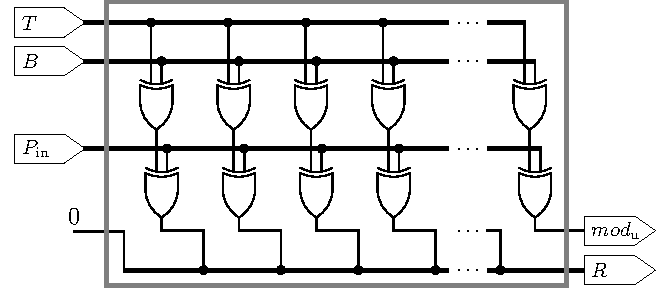
\includegraphics[width=12cm]{malu-basic}
		\figcaption{MALU - Basis ontwerp met shift}\label{figuur-implementatie-malu-basic}
	\end{center}
\end{figure}

Aangezien voor het ontwerp het veld en de modulo veelterm op voorhand bepaald zijn, is het mogelijk een zeer groot aantal XOR poorten uit het ontwerp te verwijderen. De ingang en de bijhorende $m$ XOR poorten kunnen vervangen worden door een 1 bit `modulo enable' ingang $mod_{\text{in}}$ en er worden enkel XOR poorten geplaatst voor de bits $i$ waarvoor $P_i = 1$. Hierdoor wordt het aantal ingangen drastisch verkleind en worden 
\[\Delta = m - (\text{hamm}(P) - 1)\]
XOR poorten uitgespaard, met hamm$(P)$ gelijk aan het Hamming gewicht van de binaire representatie van $P$.

In dit geval is $m = 163$ en $P = z^{163} + z^7 + z^6 + z^3 + 1$. Er zijn dus $\text{hamm}(P) - 1 = 4$ XOR poorten nodig, wat een besparing van $163 - 4 =  159$ XOR poorten oplevert ($51\%$ kleiner dan de oorsponkelijke grootte).

De resulterende schakeling is te zien in \reffig{figuur-implementatie-malu-optimized}.

\begin{figure}[h]
	\begin{center}
		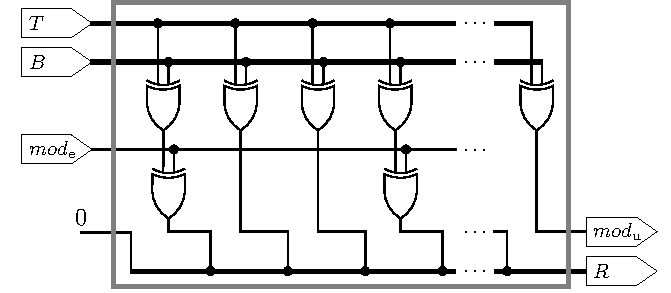
\includegraphics[width=12cm]{malu-optimized}
		\figcaption{MALU - Geoptimaliseerd ontwerp met shift}\label{figuur-implementatie-malu-optimized}
	\end{center}
\end{figure}

\section{Berekeningen in $\mathbb{F}_{2^m}$}\label{sectie-implementatie-gf2m}

De eerder ontworpen MALU schakeling laat toe optellingen te doen, maar het Miller algoritme vereist dat er ook vermenigvuldigingen worden uitgerekend. Delingen en machtsverheffingen kunnen met behulp van vermenigvuldiging berekend worden en dienen dus niet rechtstreeks ge\"implementeerd te worden. Indien dus zowel optellingen als vermenigvuldigingen berekend kunnen worden, is alles voorhanden om de Tate pairing te berekenen.

Door toepassing van een ``shift and add'' algoritme, kan de waarde van $A \cdot B = R$ berekend worden met behulp van de MALU schakeling. In \refalg{algoritme-implementatie-gf2m-multiply} is te zien hoe dit juist in z'n werk gaat. Door de modulo operatie telkens op het tussenresultaat uit te voeren, is het steeds van graad $\leq m$ en kan het steeds opgeslagen worden in $T$. Op het einde moet het resultaat door $z$ gedeeld te worden, wat neerkomt op een verschuiving van alle bits met 1 plaats naar rechts.

\begin{algorithm}[h]
\dontprintsemicolon
\caption{``Shift and add'' vermenigvuldiging in $\mathbb{F}_{2^m}$}\label{algoritme-implementatie-gf2m-multiply}
\KwIn{$A, B \in \mathbb{F}_{2^m}/[P]$}
\KwOut{$R \in \mathbb{F}_{2^m}/[P]$}
\KwData{$T \in \mathbb{F}_{2^{m + 1}}$}

$T \leftarrow 0$\;
\For{$i \leftarrow m - 1$ \KwTo $0$}{
	\eIf{$A_i = 1$}{
		$b \leftarrow B$\;
	}{
		$b \leftarrow 0$\;
	}
	
	$T \leftarrow T \xor b$\;
	
	\If{degree$(T) = m$}{
		$T \leftarrow T \xor P$\;
	}
	$T \leftarrow T \ll 1$\;
}
$R \leftarrow T \gg 1$\;
\end{algorithm}

Indien dit algoritme in een schakeling gegoten wordt, dienen enkele toevoegingen te gebeuren. Omdat een vermenigvuldiging langer dan \'e\'en klokslag duurt, is het noodzakelijk een $start$ ingang en $ready$ uitgang te hebben. Ook moet worden bijgehouden of $A$ en $B$ opgeteld of vermenigvuldigd dienen te worden. Deze functie wordt vervuld door het register $mode$. Ten slotte moet het mogelijk zijn om $R$ in $T$ op te slaan, zodat het juiste resultaat niet verloren gaat.

Bij het hoog gaan van $start$, wordt nagegaan wat de waarde van $mode$ is. Indien het om een optelling gaat, wordt $A$ opgeslagen in $T$, anders wordt $T \leftarrow 0$ zoals in \refalg{algoritme-implementatie-gf2m-multiply}. Bij een optelling is het resultaat na \'e\'en klokslag beschikbaar aan de uitgang van het MALU blok. Het dient dan enkel nog 1 bit naar rechts verschoven te worden, net zoals moet gebeuren op het einde van een vermenigvuldiging.

Wanneer dit alles in rekening gebracht wordt, verkrijgt men uiteindelijk de schakeling in \reffig{figuur-implementatie-wrapper-gf2m}. Om het geheel overzichtelijker te houden, bevat register $T$ een getal in $\mathbb{F}_{2^m}$ en wordt de waarde van $T_m$ bijgehouden in het register $mod$.

\begin{figure}[h]
	\begin{center}
		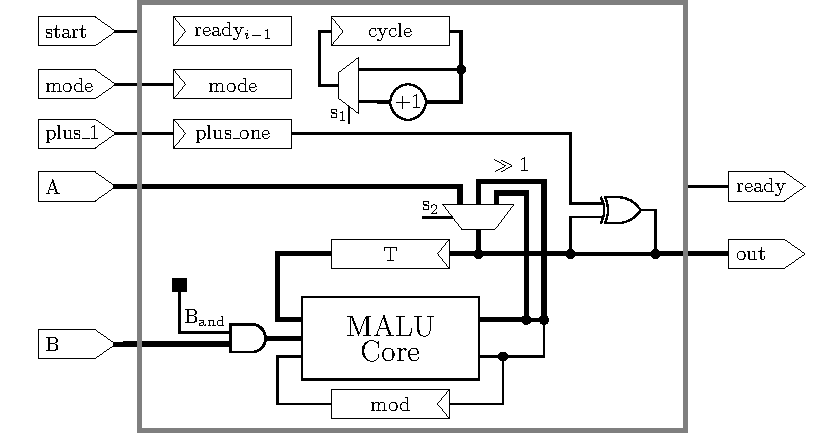
\includegraphics[width=12cm]{wrapper-gf2m}
		\figcaption{Schakeling voor berekeningen in $\mathbb{F}_{2^m}$}\label{figuur-implementatie-wrapper-gf2m}
	\end{center}
\end{figure}

